\chapter{Simulations Cosmologiques}

\newthought{Cet ouvrage est un ouvrage de théorie}. Il s'agit d'établir les quantités physiques pertinentes, les temps ou échelles caractéristiques importantes à l'évolution et l'établissement des propriétés de l'Univers : à cette fin, nous posons et analysons les équations que nous croyons pertinentes pour extraire ces informations. C'est une tâche qui généralement ne peut se faire que sous certaines hypothèses dont on sait qu'elle ne sont qu'imparfaitement satisfaites dans la réalité. Par exemple, le principe cosmologique présuppose une distribution homogène de la matière or nous savons que cela est n'est plus vrai que sur des petites échelles \sidenote{on peut mentionner les oscillations baryoniques accoustiques dans le fond diffus ($\lambda < 200$ Mpc comobile) ou bien la présence d'amas de galaxies dans l'Univers actuel ($\lambda < 1$ Mpc comobile)}.  De même, la théorie de l'instabilité gravitationnelle présentée dans le chapitre \ref{s:struct} n'est valable que dans le régime des petites perturbation, autorisant une description linéaire de la croissance des structures : pour autant nous savons qu'une galaxie présente un contraste de densité $\delta \sim 200$ qui va bien au délà des limites du régime linéaire. Il existe certes des approches permettant de dépasser le régime des petites perturbations mais elles nécessitent des conditions précises de symétries par exemple \sidenote{tel le modèle d'effondrement sphérique de Bertschinger}.


Pour toutes ces raisons, il est tout un domaine de la cosmologie physique qui vise à développer des outils de simulations numériques permettant notamment de suivre la structuration de la matière dans des régimes arbitraires de symétries et de non linéarités. Ces simulations sont essentiellement dédiées à l'étude de la \textit{dynamique} de la matière dans l'Univers en produisant des portions d'Univers synthétiques en évolution depuis les premiers instants jusqu'à nos jours. Elles reproduisent ce que nous pensons être l'histoire complexe de croissance et d'assemblage des structures : en comparant les prédictions de ces outils à la 'réalité terrain', il s'agit de tester les lois physiques qui sont utilisées et nos hypothèses sur l'état initial de l'Univers et ses propriétés. Par ailleurs ces simulations fournissent des histoires de croissances des structures qui peuvent être supplémentés de modèles supplémentaires pour explorer des physiques qui ne se limitent pas à la dynamique ou bien utilisées à des fins pratiques pour mettre au point des relevés, préparer des observations ou simuler des instruments. Ces outils numériques sont appelés \textit{simulations cosmologiques} et leurs principes les plus importants sont décrits dans ce chapitre.

\section{De la discrétisation et de la résolution}
Ces simulations sont produites par des codes informatiques devant tourner sur des ordinateurs. Ces machines possèdent des ressources finies et manipulent des quantités \textit{discrètes}, ce qui est en contradiction avec notre description habituelle du monde qui repose généralement sure une description \textit{continue} : un volume permet une infinité de positions possibles ou bien tous les instants sont accessibles à l'intérieur d'un intervalle donné. Même une quantité à priori dénombrable peu donner l'apparence d'une infinité, telle un nombre de particules qui dans des volumes cosmologiques peuvent être tout simplement gigantesque. Un traitement informatique va donc impliquer de discrétiser le temps, l'espace, la distribution de matière, etc... pour pouvoir être envisageable.
Par la suite, nous considérons la densité de matière dans l'espace $\delta(\vec x)$ : ce champ scalaire est défini en tout point de l'espace et possède donc une infinité de valeurs possibles tout en étant mesurable dans à infinité de positions possibles. 

\newthought{Un première façon} de discrétiser ce champs consiste à l'évaluer à des positions discrètes, par exemple sur une grille cartésienne de taille de maille $\Delta x$ : cette façon de faire est dite \textit{eulérienne} et permet de réduire le nombre de points où le champ est évalué tout en lui permettant toujours d'accéder à un spectre continu de valeurs. Cette façon de faire introduit en revanche un paramètre de résolution spatiale $\Delta x$ qui va limiter notre capacité à décrire des phénomènes d'échelle caractéristique proche ou inférieure à cette longueur. On pourra limiter l'influence de ce paramètre de résolution en adoptant par exemple des grilles non cartésiennes, non homogènes ou non statique mais on ne pourra jamais la faire disparaître.

\newthought{Une seconde façon} de procéder consiste à découper la matière en quanta souvent appelés \textit{particules}, qui représente une quantité prédéfinie de matière se déplaçant librement dans l'espace. Cette description est dite \textit{lagrangienne} et permet d'accéder à tous les points de l'espace de façon continue. En revanche elle introduit également un élément de résolution, en masse cette fois ci correspondant à la masse de la particule $m$ : en un point de l'espace, la quantité matière ne pourra augmenter progressivement depuis zéro qu'en 'empilant' des particules à cet endroit, d'abord $m$ puis $2m,3m$ etc... Par ailleurs cette discrétisation en quanta peut introduire du bruit si une quantité de matière donnée n'est représentée que par un faible nombre de particules. Enfin, comme pour la résolution spatiale mentionnée précédemment, cette résolution en masse nous limite dans la description de phénomène opérant dans des objets de masse inférieure à cette valeur.

\newthought{Concernant le temps} le même problème se pose: les techniques de résolution approchée d'équations différentielles nécessite généralement de raisonner sur des durées courtes par exemple pour satisfaire au mieux des approximations d'ordre linéaire ou de bas ordre. Il faut donc découper les durées d'intérêts en \textit{pas de temps} $\Delta t$ qui à nouveau nous limite quant à la description de phénomènes plus rapide que cette résolution temporelle. Une simulations numériques tachera donc de suivre l'évolution de champs discrétisés sur des grilles (dans une approche eulérienne) ou en particules (dans une approche lagrangienne), en les mettant à jour tous les $Delta t$ jusqu'à ce que la durée voulue soit couverte. Notons que les 2 approches mentionnées (grille ou particules) possèdent chacun leurs avantages et leurs inconvénients en fonctions des champs considérés et des équations différentielles qui leurs sont associés.


\section{Dynamique Non-Collisionelle: Matière Noire et étoiles}

Considérons dans un premier temps la composante non-collisionnelle de la matière, à savoir la matière noire et les étoiles. Dans la plupart des cas, une simulation cosmologique va décrire ces composantes sous forme de particules possédant une masse $m$, une position $\vec x_i$ et une vitesse $\vec v_i$ ( $i$ désignant la particule parmi N autres). La masse ne varie pas, tandis que positions et vitesses subissent des mises à jour régulières via la résolution du principe fondamental de la dynamique :
\begin{equation}
\frac{d \vec v_i}{dt}=\frac{1}{m} \vec{F}(\vec x_i)
\end{equation}
où $\vec{F}(\vec x_i)$ désigne la résultante des forces à la position $\vec x_i$. Pour une composante non collisionelle, cette résultante est uniquement le fruit de la force de gravitation. Un schéma de mise à jour simple peut prendre pour point de départ la discrétisation suivante \sidenote{par la suite on négligera la forme vectorielle des positions et vitesses en se ramenant à un problème 1D. La généralisation à 3D ne posant pas de difficultés.}:
\begin{equation}
\frac{v_i^{p+1}-v_i^{p}}{\Delta t}=\frac{1}{m} {F}(x_i^p)
\end{equation}
et permet d'évaluer la vitesse $v_i^{p+1}$ à l'instant $t^{p+1}=t^p+\Delta t$ comme suit:
\begin{equation}
v_i^{p+1}=v_i^{p}+\frac{\Delta t}{m} {F}(x_i^p).
\end{equation}
Par ailleurs, ayant $dx/dt=v$, on obtient aisément la formule de la mise à jour de la position:
\begin{equation}
x^{p+1}_i=x^{p}_i+\Delta t v_i^{p+1}.
\end{equation}
Ce schéma d'avancement simple est l'une des formes du \textit{schéma d'Euler} : s'il a le mérite de la simplicité, à l'usage il présente des inconvénients en terme de stabilité ou de précision qui nécessitent de manipuler des pas de temps $\Delta t$ particulièrement courts. D'autres schémas plus complexes existent garantissant une meilleure stabilité ou précision, par exemple le \textit{leapfrog}:
\begin{eqnarray}
v_i^{p+1/2}&=&v_i^{p-1/2}+\frac{\Delta t}{m} {F}(x_i^p)\\
x^{p+1}_i&=&x^{p}_i+\Delta t v_i^{p+1/2}
\end{eqnarray}
où l'on voit que vitesse et position sont évaluée de façon désynchronisée avec un décalage de $\Delta t/2$. L'un des mérites de cette méthode est son invariance par renversement du temps \sidenote{on parle de schéma symplectique} : en appliquant une mise à jour de $-\Delta t$ le leapfrog permet de retrouver la position $x^p$ à partir de $x^{p+1}$. Le schéma d'Euler ne possède pas la même propriété à cause du terme de force qui passe de ${F}(x_i^p)$ à  ${F}(x_i^{p+1})$ selon qu'on aille dans un sens ou l'autre. 

\newthought{La dernière inconnue} est l'expression de la force en tout point de l'espace ${F}(x_i^p)$. Plusieurs techniques ont été développées depuis les années 70 mais peuvent être rapidement regroupée en 2 familles. La première repose sur un principe de sommation : on dispose des positions $x_i$ de toutes les $N$ particules, on peut donc calculer la force appliquée sur la particule $j$ en sommant toutes les forces individuelles qui s'appliquent dessus \sidenote{on suppose que toutes les particules sont de masse $m$. $r_{ij}$ désigne la distance entre les particules i et j, tandis que $\vec e_ij $ désigne le vecteur unitaire les reliant} :
\begin{equation}
\vec F_j=-Gm^2\sum_{i\neq j} ^N\frac{1}{r_{ij}^2}\vec e_ij. 
\end{equation}
Cette méthode est simple à mettre en place et est rigoureusement exacte, toutefois elle est extrêmement coûteuse puisqu'elle nécessite d'évaluer $N(N-1)/2 \sim N^2$ interactions : si l'on décide de multiplier par 10 le nombre de particules (pour gagner en résolution en masse et étudier de plus petits objets par exemple), cela implique 100 fois plus de calculs. Ce type de dépendance en $N$ pour le coût de calcul est tout simplement insoutenable en pratique. Pour cette raison il existe des techniques qui permettent d'accélérer ce type de sommation par exemple en subdivisant hiérarchiquement l'espace suivant une configuration arborescente. Dans ces approches, une région distante (et donc peu influente) est vue avec peu de détails en regroupant les particules qui s'y trouve en 'macro-particules' moins nombreuses ce qui réduit le cout informatique de la sommation : on peut montrer que le nombre d'interactions suit une loi en $N\log N$, bien plus soutenable. Pour finir, remarquons que la formule de sommation peut diverger si certaines particules sont trop proches l'une des autres avec $r_{ij}\rightarrow 0$ : en pratique il est d'usage de lisser la force de gravitation sur un échelle $\epsilon$ :
\begin{equation}
\vec F_j=-Gm^2\sum_{i\neq j} ^N\frac{1}{r_{ij}^2+\epsilon^2}\vec e_ij. 
\end{equation}

La seconde famille de méthode pour l'évaluation de la force passe par l'estimation du champ potentiel gravitationnel $\phi(\vec x)$ sur une grille (très généralement) cartésienne. Force et potentiel dérivent l'un de l'autre :
\begin{equation}
\vec F (\vec x) =-\nabla \phi(\vec x)
\end{equation}
tandis que le potentiel peut être évalué en résolvant l'équation de Poisson à partir du champ de la densité massique $\rho(\vec x)$:
\begin{equation}
\Delta \phi(\vec x) = 4\pi G \rho(\vec x).
\label{e:poissPM}
\end{equation}
Connaissant la position $\vec x_i$ de toutes les particules, on peut évaluer la densité  $\rho(\vec x)$ en tous les points d'une grille et donc le potentiel $\phi(\vec x)$ puis la force $\vec F(\vec x)$. Connaissant la force en tous les points d'une grille, on peut alors la projeter aux positions désirées à savoir les positions $\vec x_i$ de toutes les particules.
\begin{figure}[htbp]
	\centering
		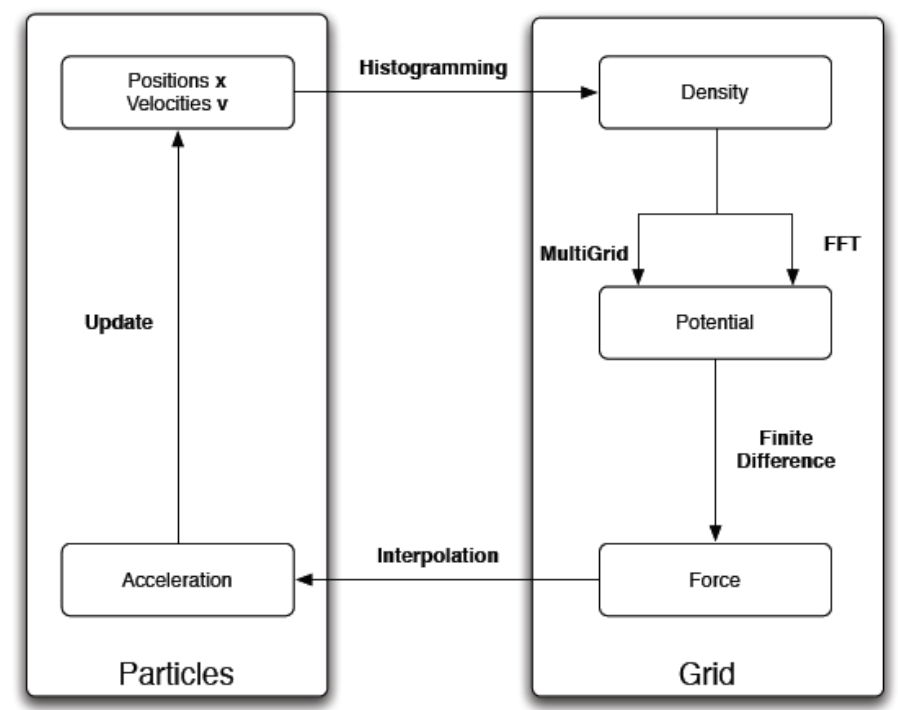
\includegraphics[height=6cm]{figs/PM.png}
	\caption{schématique de la méthode de calcul des forces sur grilles. Notez la nature hybride du schéma qui fait intervenir une description en termes de particules (ou lagrangienne à gauche) et une description en termes de champs sur une grille (ou eulérienne à droite)}
	\label{f:PM}
\end{figure}
Pourquoi se donner tant d'efforts pour évaluer la force ou le potentiel de cette façon ? La réponse réside dans la résolution de l'équation de Poisson (eq. \ref{e:poissPM}). Cette équation est fondamentalement une équation de diffusion, et nombre de méthodes ont été développée pour la résoudre efficacement et rapidement dans de nombreux contextes. Par exemple, prenons la transformée de Fourier de l'équation de Poisson et nous obtenons aisément : 
\begin{equation}
\tilde \phi(\vec k)\sim -\frac{\tilde \rho(\vec k)}{k^2}.
\end{equation} 
Si nous avons une façon simple d'évaluer les transformées de Fourier de champs connus sur une grille, il suffit d'appliquer l'équation algébrique triviale précédente pour trouver le potentiel à partir de la TF de la densité et du potentiel. Il s'avère qu'il existe des techniques de \textit{transformées de Fourier rapide} ou FFT qui ont été développées durant des décennies à des fins de traitement du signal et qui donc peuvent être facilement reprises. Grâce à la FFT, on dispose de moyens extrêmement rapide de résolution de l'équation de Poisson : en revanche l'utilisation d'une grille implique que le champ de gravitation n'est décrit qu'au mieux sur une échelle de la taille d'une cellule de la grille. Une telle échelle de coupure est inexistante à priori dans les méthodes de sommation qui permettent donc un suivi plus précis et à plus petite échelles des effondrements par exemple. L'introduction d'un lissage $\epsilon$ dans les méthodes de sommation introduisent certes une résolution limite mais ce lissage est généralement bien plus petit que la taille d'une cellule (environ 10 fois plus petit en pratique).

Pour finir, considérons rapidement la différence entre particules de matière noire et étoiles, qui toutes deux sont l'objet de la dynamique non-collisionnelle. Dans les 2 cas, les méthodes exposées ici sont appliquées de façon identique, les deux fluides diffèrent en ce que leurs membres n'évoluent pas de la même manière. Les particules de matières noires n'évoluent pas, leur masse individuelle reste constante, leur nombre initial fixe la quantité de matière noire et il n'a pas d'annihilation ni de création de telles particules. Les étoiles évoluent: elles doivent apparaître lorsque les conditions s'y prêtent et elles peuvent voir leur masse évoluer : en effet une particule 'stellaire' constitue en pratique un amas stellaire  de plusieurs centaines d'étoiles à plusieurs millions de masse solaires. Elles représentent donc davantage une population qu'une étoile individuelle en tant que tel : lorsque la partie étoile massive de ces amas explose en supernovae, la masse est rendue au milieu interstellaire au bout de quelques millions d'années et numériquement cela peut correspondre à une masse variable de particule. Notons toutefois qu'il existe toujours au sein de ces particules stellaire une composante 'étoile de faible masse' à durée vie supérieure au temps de Hubble: de façon générale une particule stellaire voit sa masse diminuer mais ne peut complètement disparaître du fait de cette population à grande durée de vie.

\section{Hydrodynamique}
\newthought{En contrepoint} de la dynamique non-collisionnelle, les codes de simulation numériques peuvent également suivre la dynamique du gaz présent dans l'Univers. Ces baryons ne représentent certes que $\sim 18\%$ de la matière disponible mais ils sont observables ou bien sont à l'origine des étoiles qui sont également observables : par conséquent ils permettent une comparaison plus directe des résultats simulés aux observations. Par ailleurs au centre des galaxies, le gaz peut être dominant et sa dynamique est suffisamment différente de celle de la matière noire et des étoiles pour devoir être modélisée indépendamment.

\newthought{Le jeu d'équation} à résoudre est connu, ce sont les équations d'Euler\sidenote{représentées ici à 1D. On y distingue l'équation de la conservation de la masse et de l'impulsion. $\rho(x,t)$ désigne la densité de gaz, $v(x,t)$ sa vitesse, $P(x,t)$ sa pression et $\phi(x,t)$ le potentiel gravitationnel.}:
\begin{eqnarray}
\frac{\partial \rho}{\partial t}+\frac{(\partial \rho v)}{\partial x}&=&0\\
\frac{\partial v}{\partial t} + v \frac{\partial v}{\partial x}&=&-\frac{1}{\rho}\frac{\partial P}{\partial x}-\frac{\partial \phi}{\partial x}
\end{eqnarray}
La première équation indique que la densité ne varie que sous l'effet du flux de masse ($\frac{(\partial \rho v)}{\partial x}$) tandis que la seconde indique que l'impulsion varie sous l'effet du flux de moment ($ v \frac{\partial v}{\partial x}$) et des forces de pression ($\frac{\partial P}{\partial x}$)  et de gravitation ($\frac{\partial \phi}{\partial x}$) \sidenote{il s'agit juste d'une formulation alternative du principe fondamental de la dynamique}.

Ces équations peuvent être toutes deux écrites sous une forme \textit{conservative}:
\begin{eqnarray}
\frac{\partial \rho}{\partial t}+\frac{(\partial \rho v)}{\partial x}&=&0\\
\frac{\partial \rho v}{\partial t}+\frac{(\partial \rho v v)}{\partial x}&=&-\frac{\partial P}{\partial x}-\frac{\partial \phi}{\partial x}\\
\frac{\partial E}{\partial t}+\frac{(\partial E v)}{\partial x}&=&-v \frac{\partial P}{\partial x}-v\frac{\partial \phi}{\partial x}
\end{eqnarray}
auquel nous avons ajouter l'équation de conservation de l'énergie $E$. Ces 3 équations suivent une structure similaire, typique d'équations de conservations d'une quantité $A$ avec un terme source:
\begin{equation}
\frac{\partial A}{\partial t}+\frac{\partial F(A)}{\partial x}=S(A).
\label{e:cons}
\end{equation}
Dans les 3 cas, une quantité $A$ est modifiée sous l'effet d'un flux $F(A)$, qui déplace la quantité en question, et d'un terme source qui modifie $A$ sans déplacement. Dans le cas de la densité, ce terme source est strictement nul ce qui indique une conservation stricte de la masse, dans le cas de l'impulsion, ce terme source est constitué des forces qui s'exercent sur le fluide et dans le cas de l'énergie il est finalement constitué du travail de ces même forces.

La façon la 'plus naturelle' de résoudre des équations du type de Eq. \ref{e:cons} est de considérer un volume fini, comme celui d'une cellule cubique et de mesurer les flux des quantités conservées (densité, impulsion et énergie) au travers des faces de cette cellule. Intuitivement, le flux mesuré au travers d'une face dépend des valeurs physiques de part et d'autre de cette face : la procédure qui permet de trouver le flux de $A$ connaissant $A$ de part et d'autre de l'interface s'appelle une \textit{resolution de problème de Riemann}.

 Il existe nombre de façons de résoudre un problème de Riemann, avec des niveaux d'approximations plus ou moins importants. Soit par exemple $F(A_{i+1/2})$, le flux existant entre 2 cellules successives $i$ et $i+1$ alors résoudre le problème de Riemann revient à trouver $\mathcal R$ tel que:
 \begin{equation}
 A_{i+1/2}=\mathcal{R}(A_i, A_{i+1/2}).
 \end{equation}
 Une façon simple de procéder revient à comparer les 'vents' dans les cellules adjacentes en comparant leurs vitesses: si $v_i>v_{i+1}$ le vent vient de la cellule $i$ et on peut considérer que la valeur de $A$ à l'interface est dominée par $A_i$. Cette procédure dite \textit{upwinds} va par exemple assigner:
  \begin{equation}
 A_{i+1/2}=\mathcal{R}(A_i, A_{i+1/2})\sim A_i
 \end{equation}
 et donc $F(A_{i+1/2})\sim F(A_{i})$. On peut toutefois montrer que ce type de schéma est soit extrêmement diffusif soit particulière instable et il existe toute une littérature de schéma de plus haut niveau plus ou moins adaptés en fonction du problème que l'on cherche à résoudre.
 
 Connaissant le flux en $i-1/2$ et $i+1/2$, la quantité $A$ peut être mise à jour par le même type de différence finie que celle utilisée précédemment pour le déplacement de particule non-collisionelle :
 \begin{equation}
 \frac{A_i^{^p+1}-A_i^p}{\Delta t}=-\frac{F(A_{i+1/2}^p)-F(A_{i-1/2}^p)}{\Delta X}+S(A_i^p)
 \end{equation}
 ou bien
 \begin{equation}
 A_i^{^p+1}=A_i^p-\Delta t \frac{F(A_{i+1/2}^p)-F(A_{i-1/2}^p)}{\Delta X}+\Delta t S(A_i^p).
 \end{equation}
Notez que cette mise à jour à l'instant $p+1$ ne nécessite la connaissance que des données à l'instant $p$ et tous les termes du membre de droite sont évalués à cet instant. Cette approche est dite \textit{explicite} et n'est que conditionnellement stable. Si le pas de temps $\Delta t$ est trop important, une amplification des erreurs s'opère la stabilité n'est garantie que si la condition de Courant est satisfaite :
\begin{equation}
\frac{\Delta x}{ \Delta t}> v.
\end{equation}
Cette équation traduit que la vitesse numérique, la vitesse de mise à jour, doit être supérieure à la vitesse typique du processus physique que l'on cherche à reproduire : pour une résolution spatiale donnée cela équivaut à mettre une limite supérieure au pas de temps choisi \sidenote{Notons que la même chose existe pour les particules de la partie précédente. Si l'on souhaite qu'une particule ne parcoure pas une trop grande distance durant un pas de temps, il faut limiter ce dernier.} Notons qu'il existe aussi une approche dite \textit{implicite} où tous les termes de mise à jour sont exprimés à l'instant $p+1$ : toutefois ces termes sont inconnus au moment du calcul et la mise à jour implique dès lors un problème typique d'inversion, souvent compliqué, en lieu et place de la simple expression algébrique obtenue ici. En revanche l'approche implicite est généralement inconditonnellement stable, ce qui permet l'utilisation de pas de temps plus grands pour simuler un problème donné.